\documentclass[12pt]{exam}
%\documentclass[12pt]{article}
\usepackage[letterpaper, margin=0.75in]{geometry}
\usepackage{graphicx}
\usepackage{enumitem}
\usepackage{booktabs}
\usepackage{amsmath}
\usepackage{tabularx}
\usepackage{color}

\begin{document}
\footer{}{Page \thepage\ of \numpages}{}

\begin{flushright}
\makebox[0.5\textwidth]{\large Name:\enspace\hrulefill}
\vspace{0.2in}

\makebox[0.5\textwidth]{\large Date:\enspace\hrulefill}
\end{flushright}

\begin{center}

\includegraphics[width=10cm]{../images/logo.png}
\end{center}

\begin{center}
\noindent{\LARGE Conceptual Physics \\ Class 12 Questions \\ April 25th, 2018 \\}
\end{center}

\clearpage

\begin{questions}
\question Is surface of the Earth an inertial frame of reference? Justify your response.

From \textit{College Physics}, Chapter 28 Question 2
\vspace{0.75in}

\question GPS satellites orbit at an altitude of about 20,000 km and at a speed of about 4000 m/s relative to the ground. In order to accurately measure position based on the travel time of a signal from a GPS satellite to a GPS receiver, we need to account for the difference between the satellite's clock and the receiver's clock. (Useful info: the radius of the Earth is 6,371 km).
\begin{parts}
\part Does special relativity predict that the satellite's clock will run fast or slow compared to a stationary clock on Earth?
\vspace{1in}
\part Does general relativity predict that the satellite's clock will run fast or slow compared to a clock on the surface of the Earth?
\vspace{1in}
\part Which effect do you think causes a greater change in the rate the clock ticks?
\vspace{1in}
\end{parts}

\clearpage
\question
Consider the following two sets of astronauts, one in a spacecraft that is experiencing uniform acceleration far from any mass and one at rest in a uniform gravitational field where the acceleration $g = -a$.

\begin{center}
				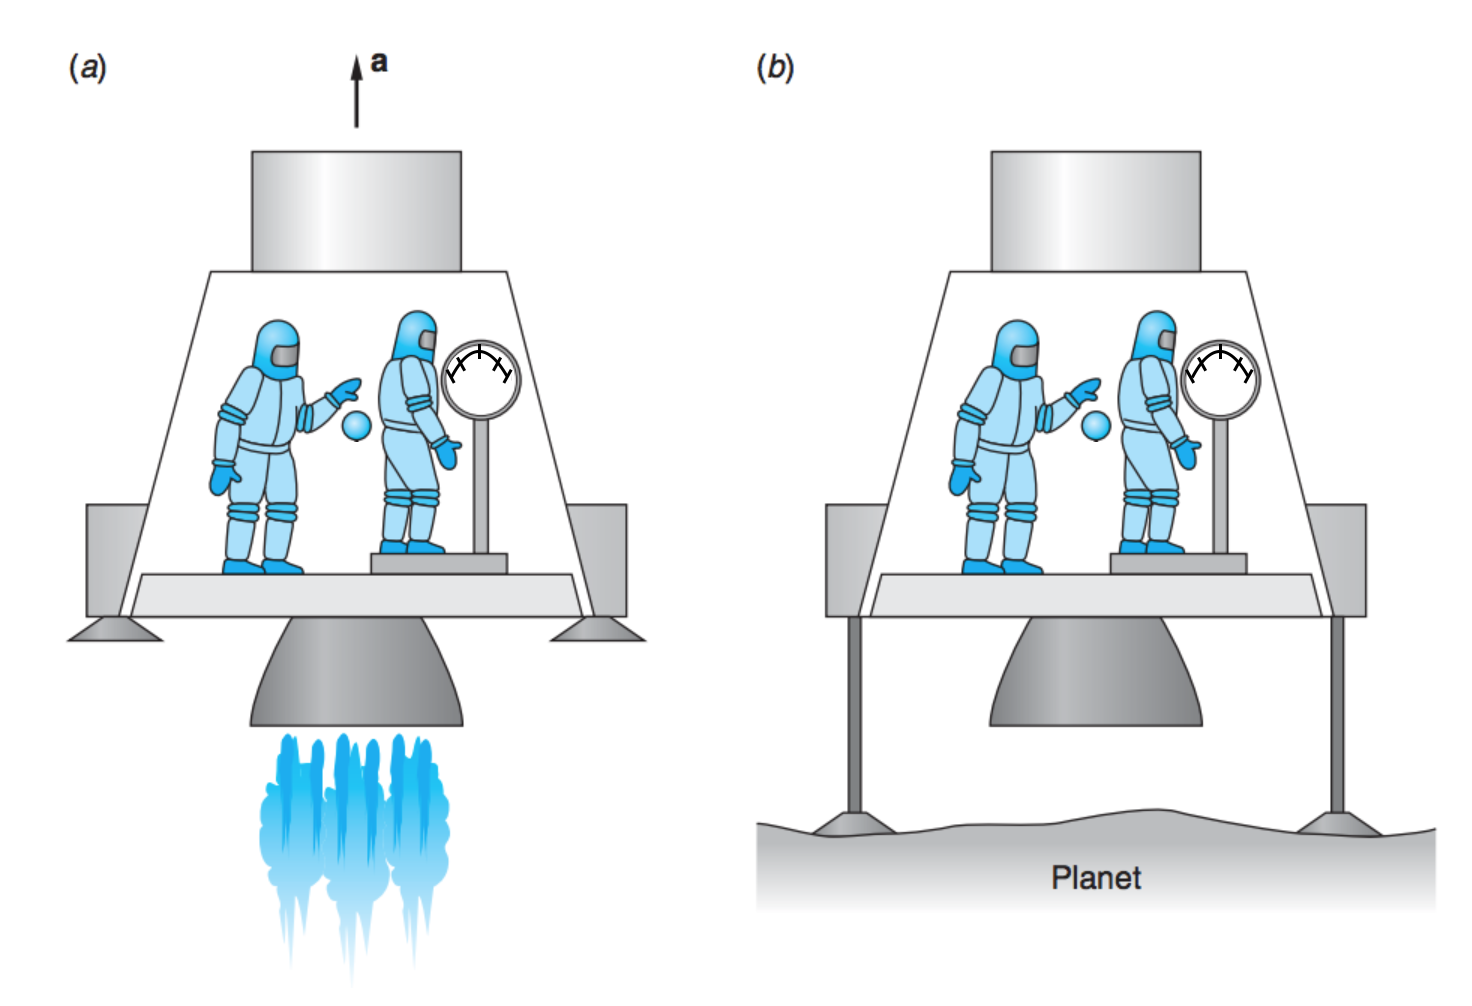
\includegraphics[width=0.7\textwidth]{../images/coop12_ep.png}
\end{center}
	\begin{parts}
	\part What will the astronauts in spaceship $a$ observe when they drop objects and stand on a scale?
	\vspace{1in}
	\part What will the astronauts in spaceship $b$ observe when they drop objects and stand on a scale?
	\vspace{1in}
	\part Is there any way to distinguish between a uniform gravitational field and a uniformly accelerated reference frame?
	\vspace{1in}
	\end{parts}
	
\clearpage
\question In order to understand the gravitational redshift and time dilation, we can determine the shift of a light pulse in an accelerating reference frame using the Doppler effect from special relativity, and then relate that to a reference frame in a gravitational field.

Consider the following two spacecrafts, one, $S$, at rest in a uniform gravitational field and one, $S'$, accelerating upwards with an acceleration $a = -g$, far from any mass. These spacecrafts contain two identical light sources located at $A$ and $A'$ and detectors at $B$ and $B'$. At time $t=0$, $S'$ begins to accelerate and an atom in the source $A'$ emits a light pulse of its characteristic frequency $f_0$.
\begin{center}
				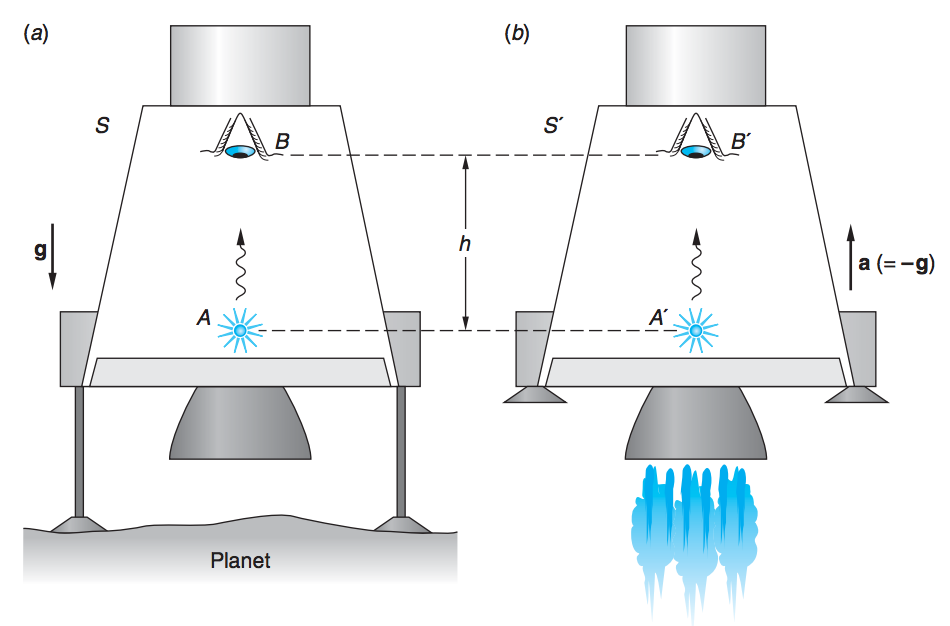
\includegraphics[width=0.7\textwidth]{../images/coop12_redshift.png}
\end{center}	
\begin{parts}
	\part During the time it takes the light pulse to travel from $A'$ to $B'$, what happens to the velocity of $B'$ relative to the location where the pulse was emitted?
	\vspace{0.5in}
	\part Does $B'$ detect the light pulse as redshifted or blueshifted?
	\vspace{0.5in}
	\part According to the equivalence principle, there is no difference between $S$ and $S'$ so $B$ must detect the same frequency shift as $B'$. However, the spacecraft in $S$ is not moving so the observed shift cannot be due to the Doppler effect. Given the change in frequency observed at $B$, how does the period change? What does an observer at $B$ conclude about the clock at $A$ (\textit{i.e.}, is it running fast or slow)?
	\vspace{0.5in}
	\end{parts}

\clearpage
\question Light follows the shortest path between two points, but since spacetime is curved near massive bodies, this path is not a straight line. Another way of thinking of this is that light falls in a gravitational field just like anything else. To understand how light can fall, let's consider how light behaves in an accelerating reference frame. Imagine you are on a space station that is not accelerating and that is far from any large object. You send a beam of light into an elevator that is undergoing uniform acceleration in the $x$ direction at $t_1$.

\begin{center}
				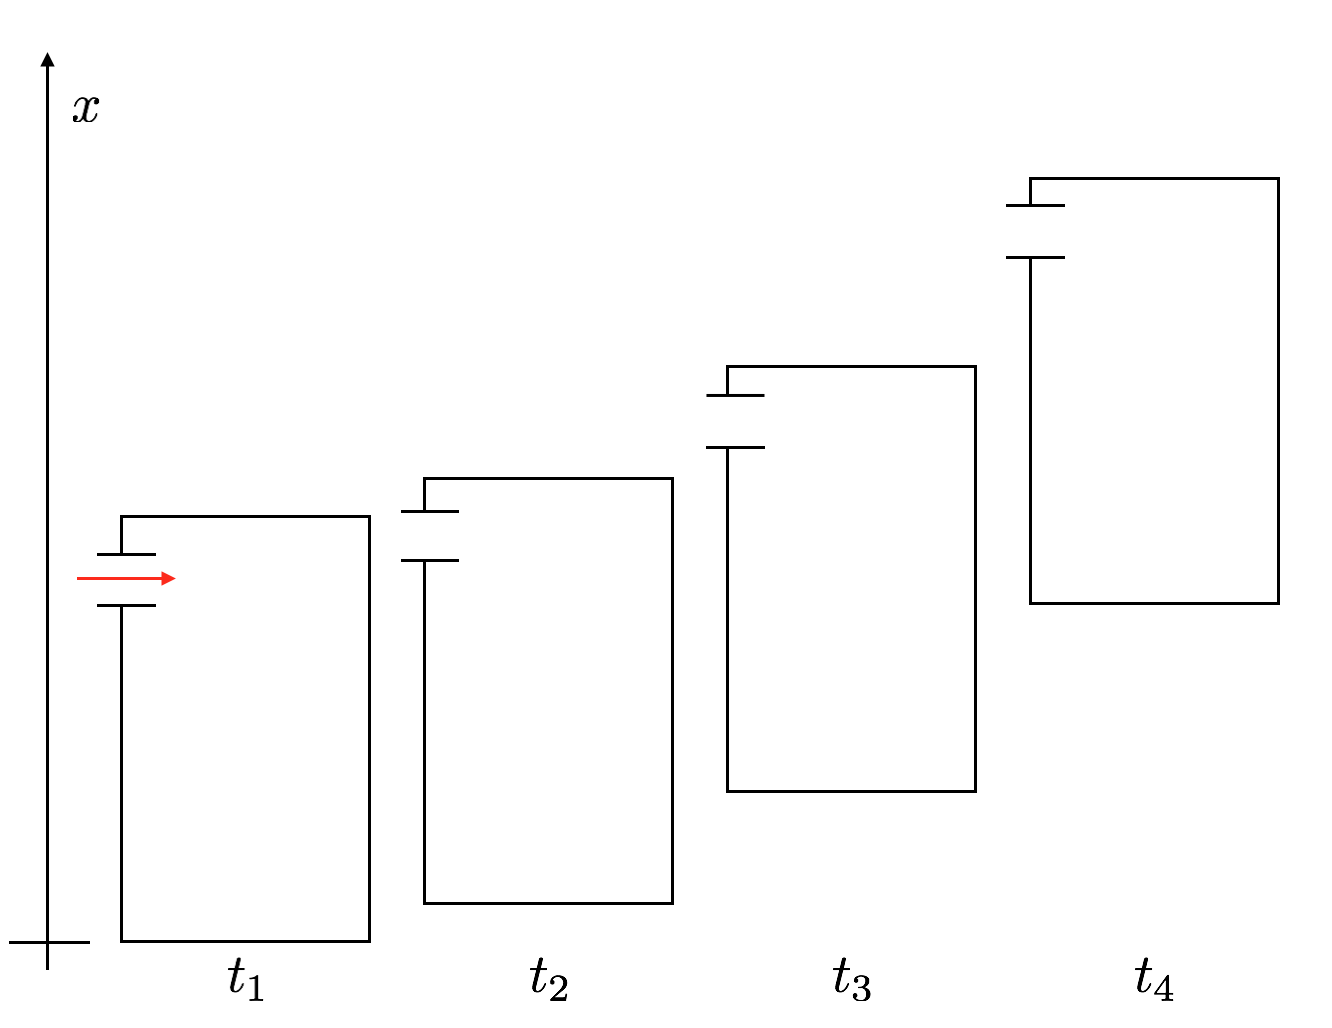
\includegraphics[width=0.7\textwidth]{../images/coop12_elevator.png}
\end{center}

\begin{parts}
\part Draw the path the beam takes in your frame of reference.
\vspace{1in}
\part How would that path look to an observer in the accelerating elevator?
\vspace{1in}

\clearpage
\part The fact that light curves around massive bodies allows us to see stars that are in the direct line of sight of the Sun and other astronomical objects. Consider the following (not to scale) drawing of light from a distant star approaching the solar system. How will its path be affected by the Sun? Where will the star appear to be, to an observer on Earth? (This was one of the first proofs of general relativity, when during the total solar eclipse of 1919 the apparent positions of several stars were observed to have shifted.)
\begin{center}
				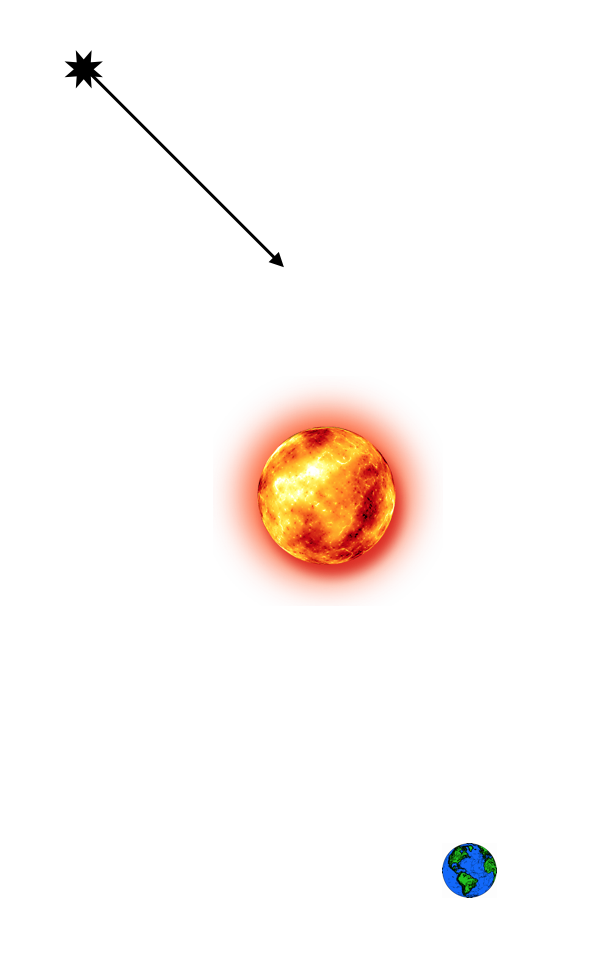
\includegraphics[width=0.35\textwidth]{../images/coop12_lightpath.png}
\end{center}
\end{parts}
	
	\question Jupiter is the largest planet in our solar system, and has many moons in orbit. If a probe landed on the surface of Europa, one of Jupiter's moons that is much smaller than Earth, and sent a radio signal with frequency of $10^4$~Hz what would the frequency appear to be:
	\begin{parts}
		\part To an observer on Earth? (higher, lower, the same?) Why?
			\vspace{1in}
		\part To an observer on Jupiter? (higher, lower, the same?) Why?
			\vspace{1in}
	\end{parts}	
	
	\clearpage
	\question The International Space Station (ISS) orbits at an altitude of about 350~km and a speed of about 8000~m/s relative to the ground. Does time run faster on the ISS than on the ground, or more slowly?
	
	From \textit{Light and Matter}, Chapter 27 Question 5
		\vspace{1in}
		
	\question As civilization grows, many people look to Mars as a potential location for a human colony. Mars is a planet with a mass much smaller than the Earth's.
	\begin{parts}
		\part Is the strength of the gravitational field on the surface of Mars greater, weaker, or the same as Earth's? Why?
			\vspace{0.75in}
		\part To an observer on Earth, would time appear to pass faster or slower on Mars?
			\vspace{0.75in}
		\part To an observer on Mars, would time appear to pass faster or slower on Earth?
			\vspace{0.75in}
		\part Assuming all else is the same (access to food, medicine, etc.) would a person on Earth have a longer, shorter, or the same life-span as a person on Mars?
			\vspace{0.75in}
		\part If the two colonies became isolated and didn't communicate for a very long time, then suddenly reconnected, which would you expect to have a longer history? Why?
			\vspace{1in}
	\end{parts}
	
\clearpage
	\question \textbf{The Twin Paradox} Two identical twins, Alice and Betty, are separated when they are very young. Alice stays on Earth, and the Betty is on a spaceship that accelerates to 99.999\% of the speed of light to visit a distant star, then comes back. For the purpose of the following questions, Earth's gravitational field is so small it is negligible.
		\begin{parts}
			\part While the ship is traveling at 99.999\% of the speed of light, does Alice perceive Betty's time to be dilated? Why or why not?
				\vspace{1in}
			\part While the ship is traveling at 99.999\% of the speed of light, does Betty perceive Alice's time to be dilated? Why or why not?
				\vspace{1in}
			\part When Betty comes back to Earth, which twin, if any, will appear to be older?
				\vspace{1in}
		\end{parts}
		
	\question From Betty's perspective, she ``time traveled" into Earth's future. Is it possible for her to travel back? If so, how could she do this? If not, why not?
		\vspace{1in}

\clearpage
	\question From the observations about the expansion of the universe, we notice that, the further objects are from us, the faster they appear to be moving. A useful analogy is an ant walking on an inflating balloon, who sees its ant friends on different parts moving further and further away. The arrows indicate their relative velocities, with longer arrows indicating they are moving apart faster.
	\begin{center}
	\input{../images/antsBalloon.pdf_tex}
	\end{center}
	\begin{parts}
		\part As the balloon expands more, the ants appear to be moving faster and faster apart, but they try to stay in contact by little ant walkie-talkies (which send radio signals to each other). After some time, they appear to be moving away from each other at the speed of light. What happens to their communication then?
			\vspace{0.5in}
		\part The distance between two points that light cannot travel due to the expansion of the universe is called the \textit{Hubble Horizon}. As the rate of expansion increases, what happens to the length of this Hubble Horizon?
			\vspace{0.75in}
		\part If the rate of expansion were to slow, what would happen to the Hubble Horizon?
			\vspace{0.75in}
		\part If the Hubble Horizon were to shrink to smaller than an atom, what would happen?
			\vspace{0.75in}
		\part If the Hubble Horizon were to shrink to smaller than an atomic nucleus, what would happen?	
			\vspace{0.75in}
	\end{parts}
	
	\question Imagine a universe which was not expanding, that existed forever and had an infinite size. In such a universe, what would the night sky look like?
		\vspace{1in}
		
	\question Where did the Big Bang happen?
		\vspace{1in}

\question Different kinds of stars emit different spectra of light. A distant star within our galaxy emits light with a wavelength that is predominantly 700~nm. It is possible for different observers to measure a different wavelength for this light.
	\begin{center}
	\input{../images/earthProbeStar.pdf_tex}
	\end{center}
	\begin{parts}
		\part What factors must be considered, which can impact the observed wavelength of light?
		\vspace{1in}
		\part To an observer on the Voyager space probe, which has exited the solar system and is millions of miles away from any object, what will the wavelength be (longer, shorter, the same, can't say)? Why?
		\vspace{1in}
		\part To an observer on Earth, what will the wavelength be (longer, shorter, the same, can't say)? Why?
		\vspace{1in}
	\end{parts}
	
	\question Clock A sits on a desk. Clock B is tossed up in the air from the same height as the desk and then comes back down. Compare the elapsed times.
	
	From \textit{Light and Matter}, Chapter 27 Question 7
	\vspace{0.75in}
	
	\question You are on a spaceship, orbiting a distant planet. There is a malfunction, with the ship, which begins to experience engine problems, and you are knocked out. When you wake up, you are locked in a room on your ship, which is continuing to malfunction and you cannot get out. However, you can feel a force of gravity and are able to stand up and move around. In this room, you have at your disposal all the latest scientific equipment and can perform any experiment (dropping balls, emitting light and detecting Doppler shifts, etc.) How can you distinguish between: (1) having crashed on the planet, and (2) the engines are accelerating the ship?
	\vspace{1.5in}

\end{questions}


\end{document}
